% Two fair dice: 36 ordered outcomes. Six sum to 7 (rust); one sums to 2 (charcoal).
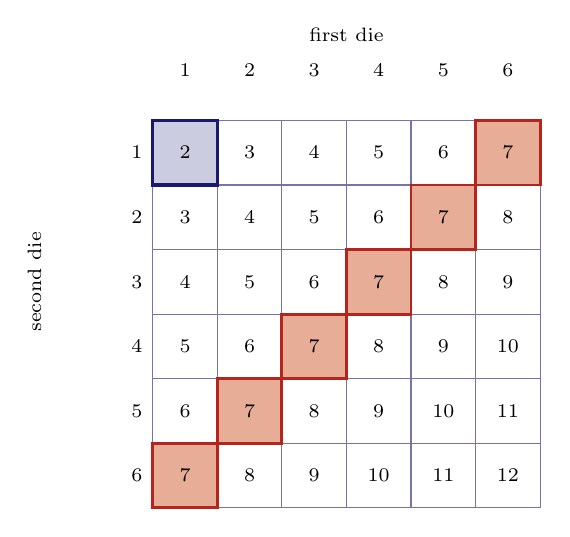
\begin{tikzpicture}[x=0.82cm,y=0.82cm,every node/.style={inner sep=0pt}]
  \node[font=\scriptsize,anchor=south] at (4.0,0.22) {first die};
  \node[font=\scriptsize,rotate=90,anchor=south] at (-0.72,-3.5) {second die};
  \foreach \i in {1,...,6} {
    \node[font=\scriptsize] at (\i+0.5,-0.22) {$\i$};
    \node[font=\scriptsize,anchor=east] at (0.85,-\i-0.5) {$\i$};
  }
  \foreach \i in {1,...,6} {
    \foreach \j in {1,...,6} {
      \pgfmathtruncatemacro{\s}{\i+\j}
      \ifnum\s=7
        \fill[BrickRed!30] (\i,-\j) rectangle ++(1,-1);
      \fi
      \ifnum\i=1
        \ifnum\j=1
          \fill[MidnightBlue!22] (\i,-\j) rectangle ++(1,-1);
        \fi
      \fi
      \draw[MidnightBlue!60,thin] (\i,-\j) rectangle ++(1,-1);
      \node[font=\scriptsize] at (\i+0.5,-\j-0.5) {$\s$};
    }
  }
  \foreach \i/\j in {1/6,2/5,3/4,4/3,5/2,6/1} {
    \draw[BrickRed,line width=1.05pt] (\i,-\j) rectangle ++(1,-1);
  }
  \draw[MidnightBlue,line width=1.15pt] (1,-1) rectangle ++(1,-1);
\end{tikzpicture}
